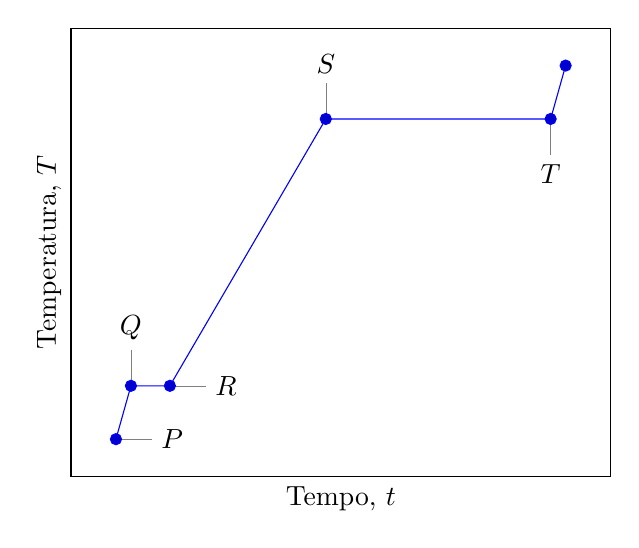
\begin{tikzpicture}
    \begin{axis}
        [
            xlabel = {Tempo, $t$},
            ylabel = {Temperatura, $T$},
            xtick=\empty, ytick=\empty,
        ]
    \addplot coordinates 
        {
        	(0,-20)
        	(5,0)
        	(18,0)
        	(70,100)
        	(145,100)
        	(150,120)
        };
    \node[coordinate,pin=right:{$P$}] 
    	at (axis cs:0,-20)   {};
	\node[coordinate,pin=above:{$Q$}] 
		at (axis cs:5,0)	 {};
	\node[coordinate,pin=right:{$R$}] 
		at (axis cs:18,0)	 {};
	\node[coordinate,pin=above:{$S$}] 
		at (axis cs:70,100)	 {};
	\node[coordinate,pin=below:{$T$}] 
		at (axis cs:145,100) {};
    \end{axis}
\end{tikzpicture}